
%(BEGIN_QUESTION)
% Copyright 2015, Tony R. Kuphaldt, released under the Creative Commons Attribution License (v 1.0)
% This means you may do almost anything with this work of mine, so long as you give me proper credit

A newly commissioned pressure control system has a problem: the controller registers a process fluid pressure of 22 PSI, but two pressure gauges connected to the same vessel both register 35 PSI.  A technician is sent to troubleshoot this problem, and decides to measure current at terminal 2 of TB-52 (located in Field Panel JB-25).  The current signal registers 15.2 milliamps DC:

$$\includegraphics[width=15.5cm]{i02551x01.eps}$$

Based on these symptoms and information contained in this loop diagram, answer the following questions:

\begin{itemize}
\item{} Where do you think the problem lies, and what sort of problem might it be?
\item{} Sketch how the technician's milliammeter should be connected in order to intercept the loop current at terminal 2 of TB-52.  Include the test lead colors (red, black) in your answer.
\item{} Identify what steps the technician (or operator) should have done prior to taking the current measurement, to ensure nothing bad (e.g. process interruption, alarms) would happen when the circuit was broken to insert the milliammeter.
\item{} Modify both the transmitter and control valve 4-20 mA loop circuits to include diodes for the purpose of convenient current measurement.
\end{itemize}

\vskip 20pt \vbox{\hrule \hbox{\strut \vrule{} {\bf Suggestions for Socratic discussion} \vrule} \hrule}

\begin{itemize}
\item{} A useful analytical technique for any DC electric circuit is to identify all electrical sources and loads in the circuit, annotate the diagram with arrowheads showing the directions of all currents, and also with ``+'' and ``$-$'' symbols (and/or curved arrows) showing the polarities of all component voltages.  Show how this helps you analyze the circuit shown in this question.
\item{} Identify other diagnostic tests you would perform on this system to further pinpoint the nature and location of the fault.
\end{itemize}

\underbar{file i02551}
%(END_QUESTION)





%(BEGIN_ANSWER)


%(END_ANSWER)





%(BEGIN_NOTES)

15.2 milliamps corresponds to 35 PSI in a 0-50 PSI transmitter range, which tells us the transmitter (PT-6) agrees with the two pressure gauges in saying that the process fluid pressure is 35 PSI.  The fault, therefore, lies with the controller's interpretation of this milliamp signal.

One possibility is that the controller input is mis-configured (e.g. LRV/URV values are set incorrectly).  Another possibility is a ground fault (short to ground) in the black wire of cable 4 pair 1 or cable PT-6 at the controller input, shunting some of the 15.2 mA signal around the controller input so that the controller doesn't see the full signal strength.  One way to further diagnose the problem is to take a similar current measurement at terminal 12 of the analog input card.

\vskip 10pt

The technician's multimeter should be connected as a {\it load}: current (conventional flow) entering the red test lead, and current exiting the black test lead.  Since current travels counter-clockwise in the transmitter loop, this means the red test lead will be on the left and the black test lead will be on the right.

\vskip 10pt

The operator should place the controller into {\it manual mode} prior to any work being done on the transmitter circuit.  If any PV alarms are configured on the controller, they should be temporarily disabled as well prior to doing the work.

\vskip 10pt

Modified loop diagram containing diodes:

$$\includegraphics[width=15.5cm]{i02551x02.eps}$$

%INDEX% Basics, control loop troubleshooting

%(END_NOTES)


